\documentclass[12pt]{article}

\usepackage{setspace}
\usepackage{hyperref}
\usepackage{graphicx}
\usepackage{url}
\usepackage{xcolor}
\newcommand\todo[1]{\textcolor{red}{#1}}

\onehalfspacing

\parskip=2ex
\parindent=2em

\title{SWEN439 Visualisation Essay \\ John Snow's Cholera Map}
\author{Hai Tran 300224467}
\date{\today}

\begin{document}
\maketitle 

%Optional abstract
\begin{abstract}

\end{abstract}
\textcolor{red}{
You will pick a visualisation and write an essay about that visualisation. 
You can do the cholera map, then show other things that were similar at the time, and for future show what visualisations came after that resemble it. Like dot maps. They would be not the main topic, but just an example of modern visualisations that are similar or you can contrast it with modern visualisations for disease spread to show how we do the same thing these days but use perhaps different visualisations.
}

\begin{itemize}
\item A clear description of the visualisation and how to read / interpret it
\item What questions does this visualisation address effectively and which does it not?
\item Is this a visualisation that is easy to use for novice viewers, or is it more intended for experts?
\item What is the history of the visualisation? Where did it come from? Where is / was it used?
\item What is the current state of research with respect to this visualisation?
\end{itemize}

\section{Introduction}

\section{The History of John Snow's Cholera Map}
\todo{ Thousands of lives were lost each year to the disease cholera in the nineteenth century. In the nineteenth century, thousands of lives had been lost due to a disease called cholera.}

The nineteenth century was plagued with a disease called cholera, thousands dying each year due to the disease. Although unknown at the time, cholera is caused by a bacteria that doubles in number every thirteen minutes, attacking the stomach and intestines \cite{channel1}. This provokes severe vomiting and diarrhea in victims, eventually causing an agonizingly death to the victim in a matter of hours \cite{heros, channel1}. During the time of the nineteenth century, 



\todo{from wiki}
During the nineteenth century, the Soho district of London had problems with filth due to the large amount of people and a lack of proper sanitary services. Many basements had cesspools underneath their floorboards that stored fecal matter. Since the cesspools were overrunning, the London government decided to dump the waste into the River Thames. This action contaminated the water supply, leading to a cholera outbreak. 

In 1854 London was gripped by cholera; many thousands were to die in the ensuing epidemic. Most doctors at the time believed that the disease was caused by foul smelling mist “miasmas” a view contested by Dr John Snow who suspected that contaminated drinking water was the cause. Snow believed that if the disease was caused by air then the incidents of disease would be evenly spread throughout the streets of London, whereas if poisoned water were the culprit, cases would cluster in locations around the source of the contamination. In order to prove his theory he drew a map of Soho marking each case of cholera with a black dot. He also marked each public water pump in the area with an “X”. By analyzing the distribution of black dots in relation to the water pumps, Snow was able to track the origin of outbreak in Soho to Broad Street. Snow immediately advised decomissioning the pump in Broad Street and very quickly the outbreaks of cholera cleared. \cite{test}

In the nineteenth century, cholera was a disease that killed many thousands a year. Today, we know that cholera is caused by a bacteria - Vibrio cholerae, which has been shaped by evolution to spread itself in a devilish manner: It provokes severe vomiting and diarrhea. If its victims live very close to each other and they don't have access to adequate sanitary conditions, it is likely that the fluids they release will contaminate sources of water or food.

Until the 1860s, most scientists were convinced that cholera was caught by breathing the stinky effluuvia that emanated from foul water and soil, or from decaying wastes. This miasma "bad air" theory of disease was based on persistent correlational observations: Contagious maladies hit poor areas harder. 

John Snow hypothesised that cholera was a waterborne disease caused by a germ. He wrote academic papers to make his case, but no one listened to him. The tide shifted when a brutal outbreak in 1854, in which hundreds of Londoners perished within a few weeks, led him to produce his famous map. \cite{heros}


2.5 million 1854, a third living in slums, up to eight to a room, 40 to a house. 
 In just three days, 127 dead in London. No one knows who is causing the disease and there is no cure. But one man is determined to stop it, physician John Snow. Entering the outbreak John Snow risked his life to find the source. Most doctors believe Cholera is carried by foul air. Snow has studied various outbreaks and is convinced Cholera is in the water. "A revolutionary insight that will turn the industrial city from a death trap into the engine of our world." 600 dead in just two weeks in London. Snow searches for a pattern, analysed the data in front of him, and made a miraculous discovery in front of him. Snow plots his findings on a map, a map of the dead. 578 in one small neighbourhood. He lists the water pumps they used, to see if there is a pattern. The map showed that all the deaths had taken place near the broad street pump. 2800 people live within 100 yards of the broad street pump, most drink its water. The authorities refuse to shut it down. Then a new victim who doesn't fit the pattern, from broad London, no where near the broad street pump. Could his hypothesis be wrong? Susanna Eley. Eley's mother moved from the area a few years ago. She preferred the water from central London, so her son sent a daily supply from the Broad Street pump. It's the proof that Snow's been searching for that the authorities can't ignore. Just three feet from an open sewer, through cracks and crevices deadly sewerage leaks into the water supply. When the authorities removed the handle from the pump, the outbreak stops. John Snow's method of mapping the spread of disease is still used today. It was a very clear and scientific approach to taking information, connecting the dots and making sense of what was happening. All the information was out there, but until John Snow, we hadn't put the pieces together yet. \cite{channel1}

It took awhile for the authorities. By 1896, the next outbreak that broke out, the authorities were convinced because of the map and told everybody to start boiling there water. That was the last time that London had seen a cholera outbreak since \cite{tedtalk}. 

He learned, for example, that the brewery and the workhouse, both near the Broad Street pump, had their own independent water sources and so escaped the outbreak largely unscathed. \cite{blog}

8th of September 1854, on the instructions of John Snow, the handle of the pump was removed. Spread through miasma: a pollution of the atmosphere. Found the people least effected were the brewery workers who were drinking beer rather than water. When he got authorities to remove the handle, it was more symbolic since the Cholera epidemic had pretty much burnt itself anyway. The real significance of John Snow's story was that its the birth of epidemiology, the birth of statistical analysis, and it shows how many lives you can save, improve conditions with proper conditional surveys. \cite{youtube}

\section{John Snow's Cholera Map}


On it, thin, tiny strokes represent deaths and circles show the locations of water pumps. The message of the map is clear: Deaths cluster around the Broad Street well, which had been poisoned by fecal matter from a sick baby (this was discovered later). John Snow not only drew the map, but he also convinced the local authorities to remove the handle of the water pump, an action that stopped the outbreak. Snow, many have said, changed medicine forever. \cite{heros}

Each black bar represented a death in the neighbourhood \cite{tedtalk}. As you get further away from the pump, the deaths seem to get less and less frequent. So you can see something poisonous emanating out of this pump on the map. 

The deaths at each address are indicated by the little horizontal lines, stacked up from the street like a pile of little corpses. Snow has made the map big enough to include the locations of the other water pumps in the vicinity, clearly showing a drop-off in cholera deaths where houses are nearer to a different pump. Visualizing his data allowed Snow to investigate abnormalities in the outbreak. \cite{blog}

    \begin{figure}
    \centering
    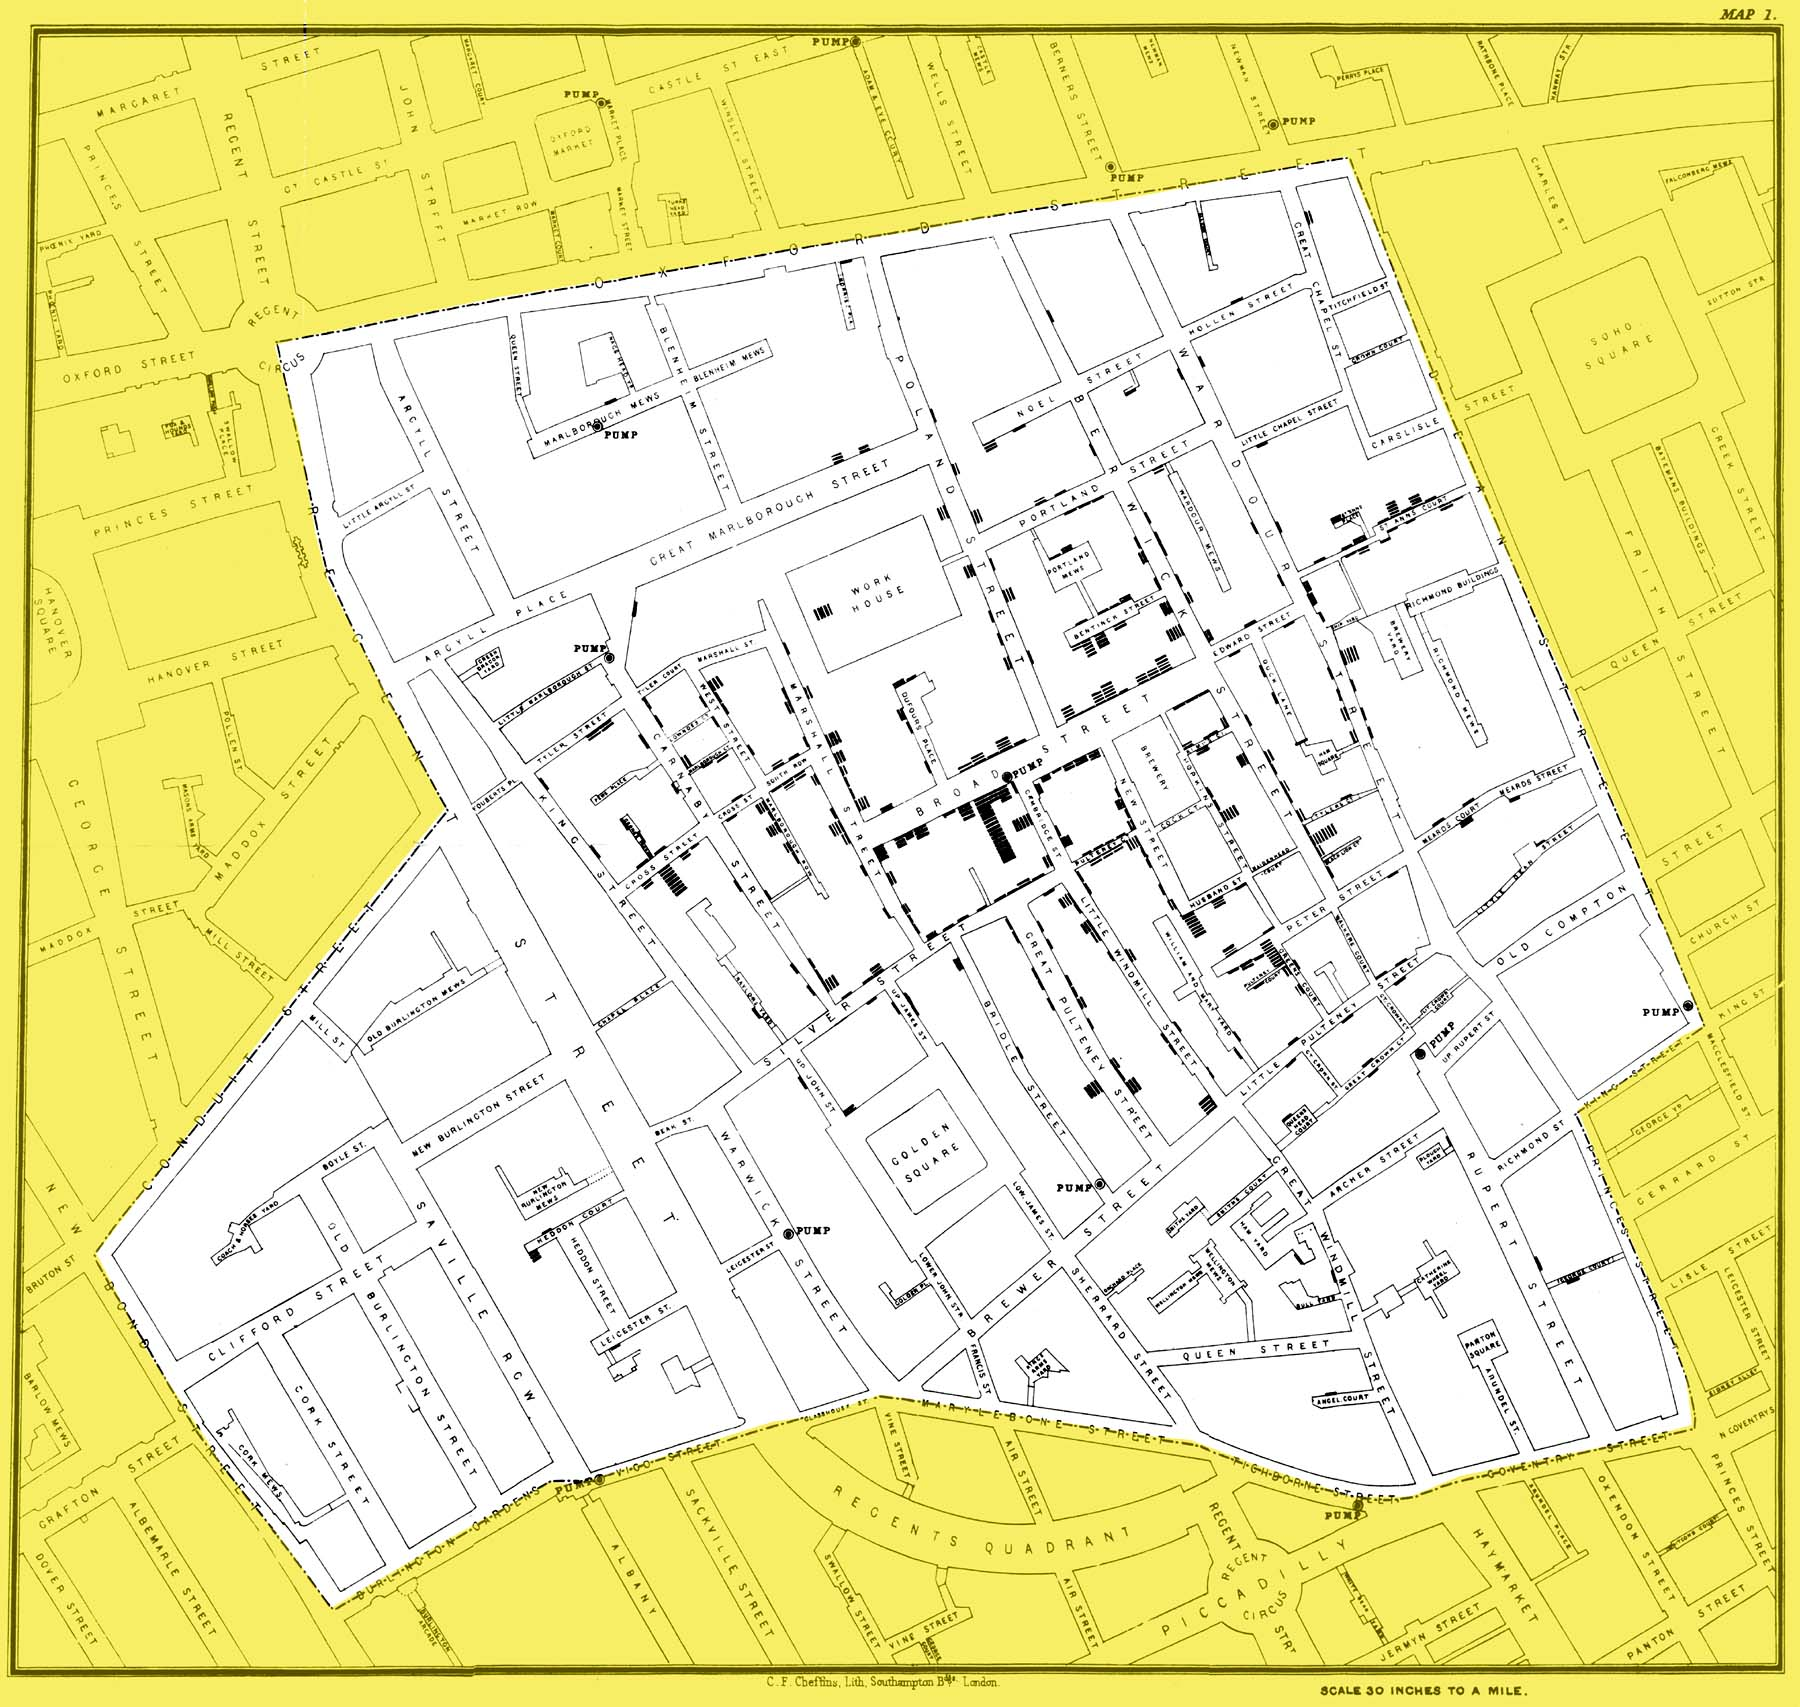
\includegraphics{snowmap_1854}
    \caption{Caption}
    \label{fig:snow}
    \end{figure}
    
    \begin{figure}
    \centering
    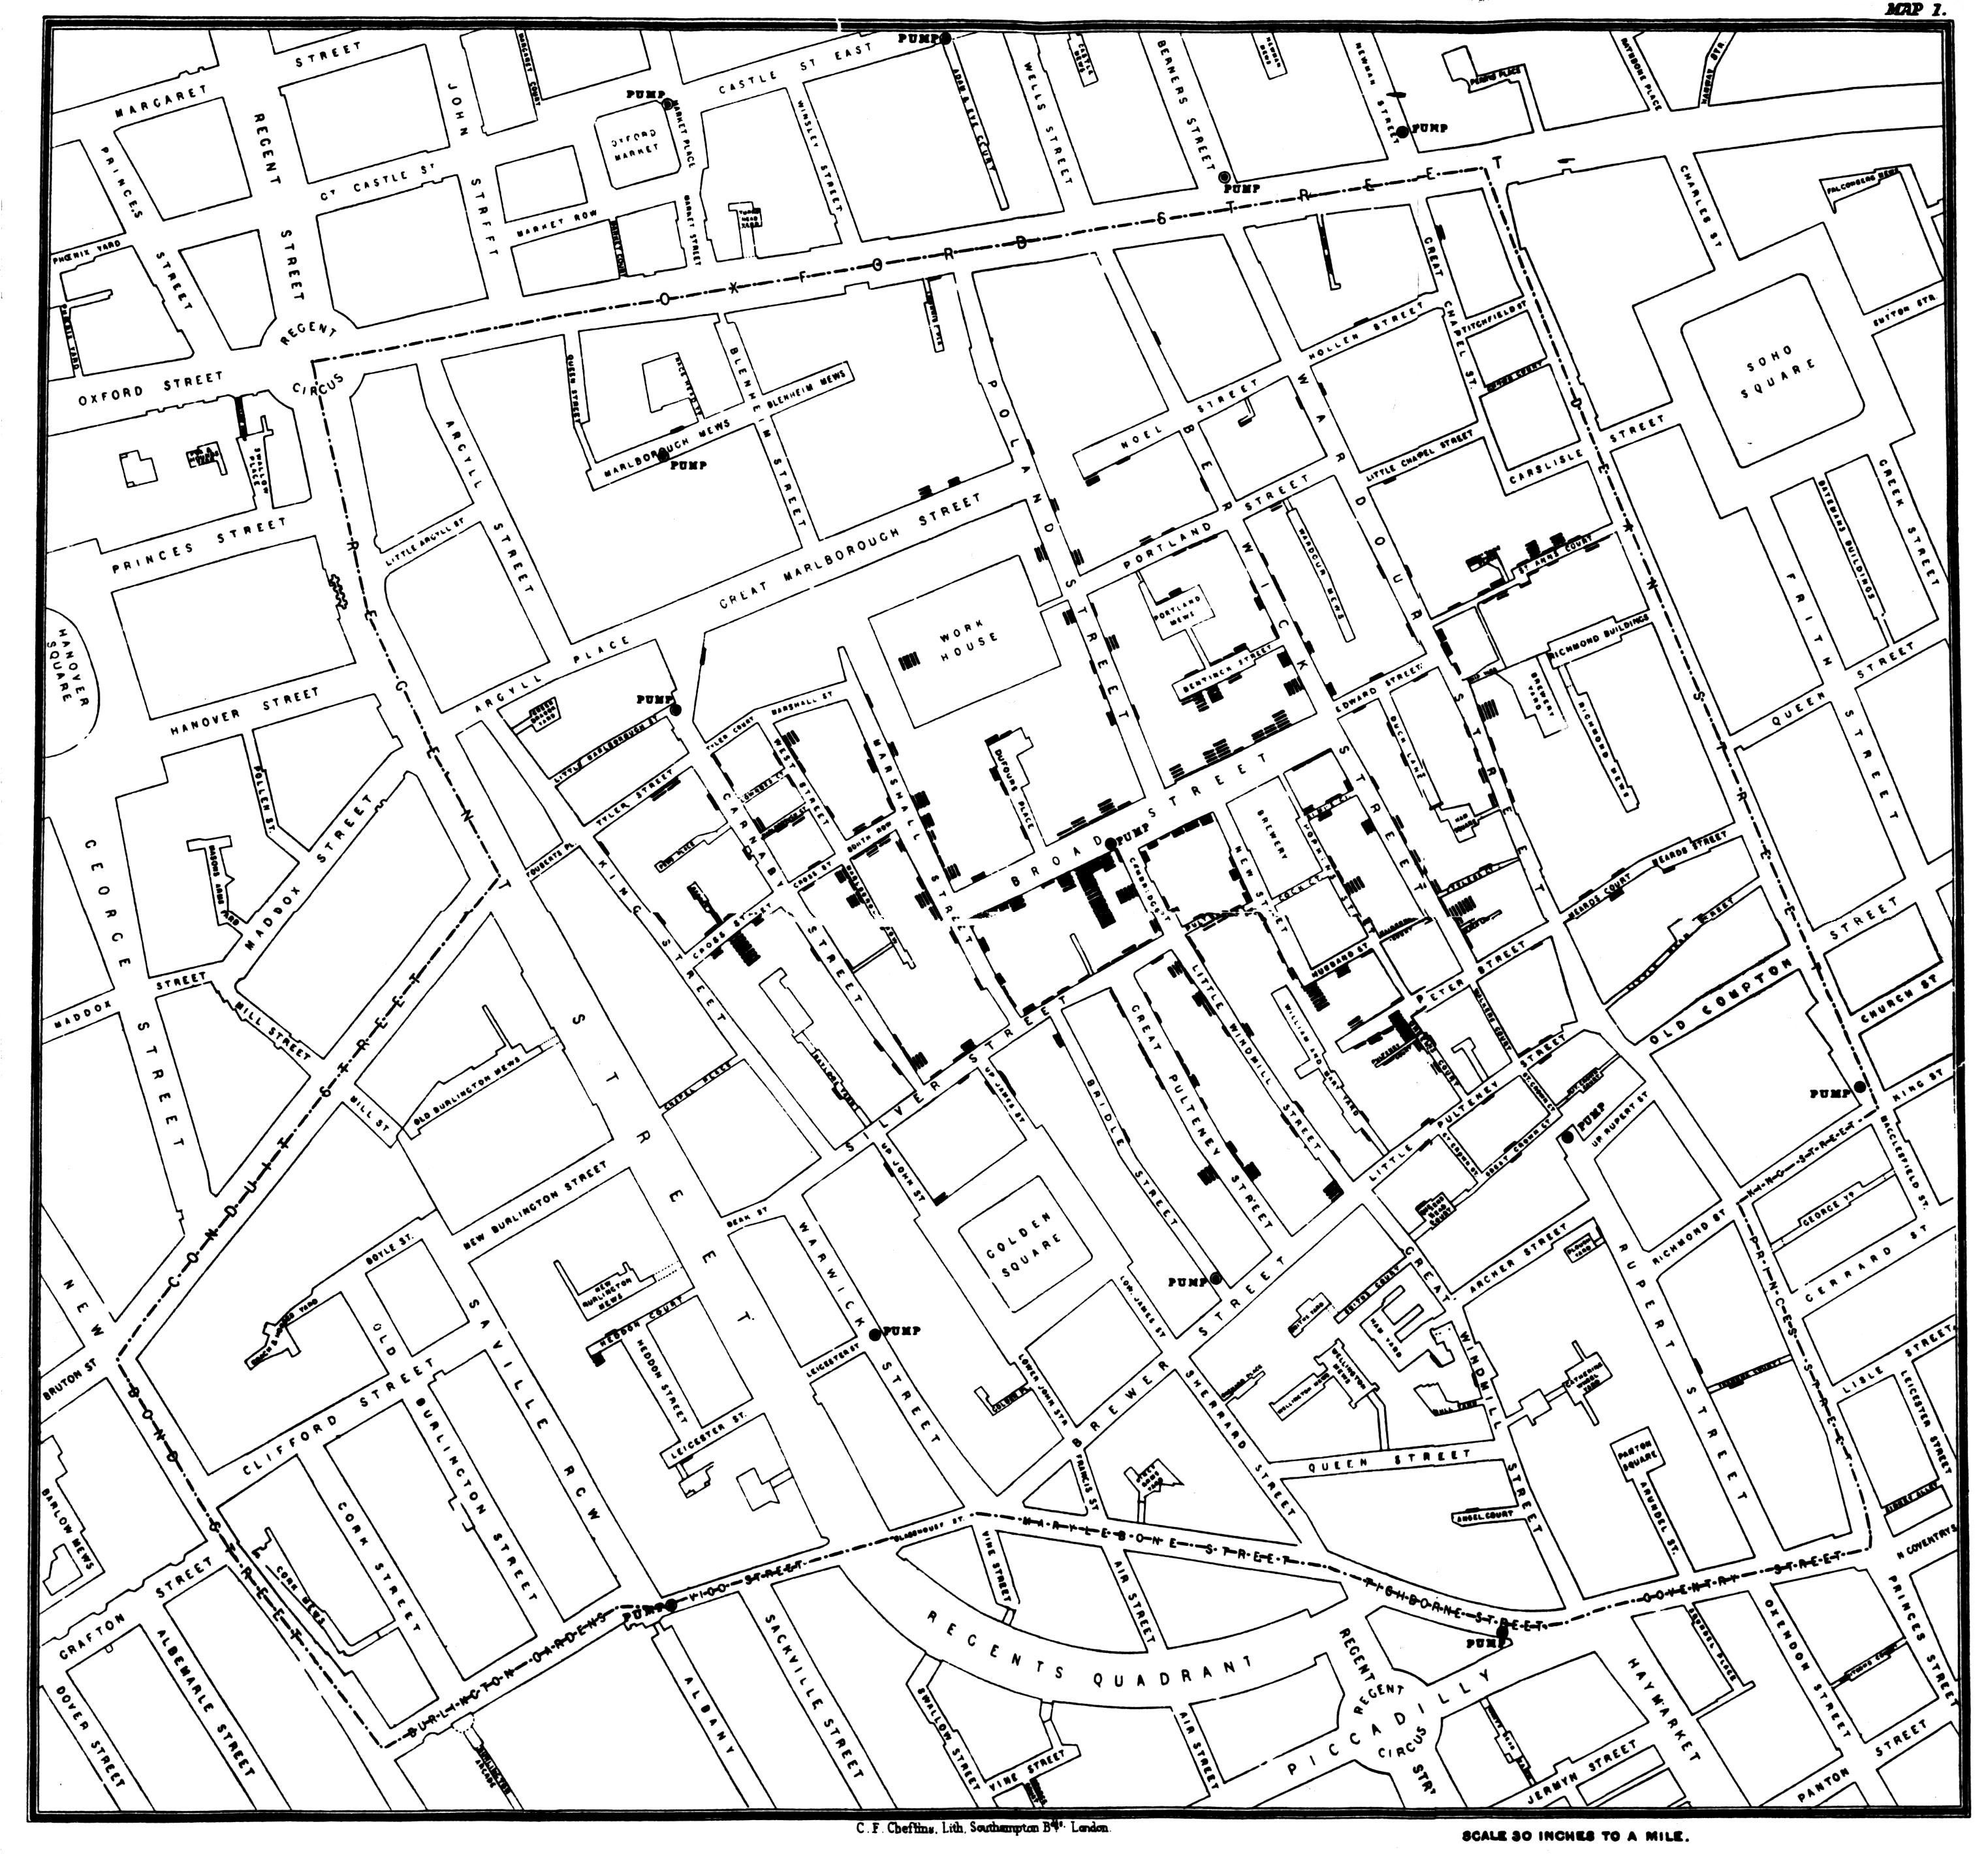
\includegraphics[scale=0.1]{Snow-cholera-map-1}
    \caption{John Snow's Cholera map}
    \label{fig:snow}
    \end{figure}



\section{Weaknesses}

Edward Tufte, a godfather of information display, analyzes this map in his 1997 book, Visual Explanations. Tufte points out that as a dot map, 2 Snow’s visualization is implicitly assuming that the population in the area is uniformly distributed. In other words, a house without any deaths means that the inhabitants of that house successfully avoided cholera, not that the house sits empty. But even with that shortcoming, Tufte praises the map’s usefulness. \cite{blog}

\section{The Impact/Significance/Influence of Snow's Cholera Map}

His work addressed an ongoing medical debate — in what is widely regarded as one of the most important early examples of epidemiology, he clearly linked cholera’s spread to water instead of air. \cite{blog}

This map that changed the way the world understood cholera. It forced London to realise it needed to build a sewage system to fix itself and end cholera outbreaks. This map makes my top 5 because it was used to convince people of the need for change. \cite{top5}

His map is not only an important historical moment in public health, but also a breakthrough in the visual display of information. By showing abstract medical statistics within a geographic image, a pattern of illness distribution was made visible in a way that pointed to its cause. Today we call such information visualisations Graphic Information Systems (GIS for short). \cite{test}

Steven Johnson, in his book “The Ghost Map” about the London cholera epidemic and efforts to stop it, notes that Snow’s was not the first map to chronicle cholera outbreaks, or even this particular cholera outbreak. \cite{history}

\todo{could be moved to history?}
Among the earliest examples of disease mapping were
two spot maps prepared by Valentine Seaman to illustrate
the distribution of yellow fever in New York
towards the close of the eighteenth century. Shapter2, in
his History of the Cholera in Exeter in 1832 included a dot
map showing the distribution of deaths caused by
cholera. (Figure 1). \cite{howe1970some}

“Part of what made Snow’s map groundbreaking was the fact that it wedded state-of-the-art information design to a scientifically valid theory of cholera’s transmission. It was not the mapmaking technique that mattered; it was the underlying science that the map revealed,” Johnson writes. \cite{history}

It's possible to solve these problems, if we look at the empirical evidence such as the map. ``It's a  map of deaths that ended up creating a whole new way of life, a life that we are enjoying today." \cite{tedtalk}

\todo{from wikipedia}
Snow's study was a major event in the history of public health and geography. It is regarded as the founding event of the science of epidemiology.


\section{Modern Visualisations}

\section{Conclusion}


% \bibliographystyle{IEEEtranN}
% \bibliographystyle{ieeetr}


\bibliography{mybib}
\bibliographystyle{ieeetr}

\end{document}